
\begin{figure*}[t]
\center
    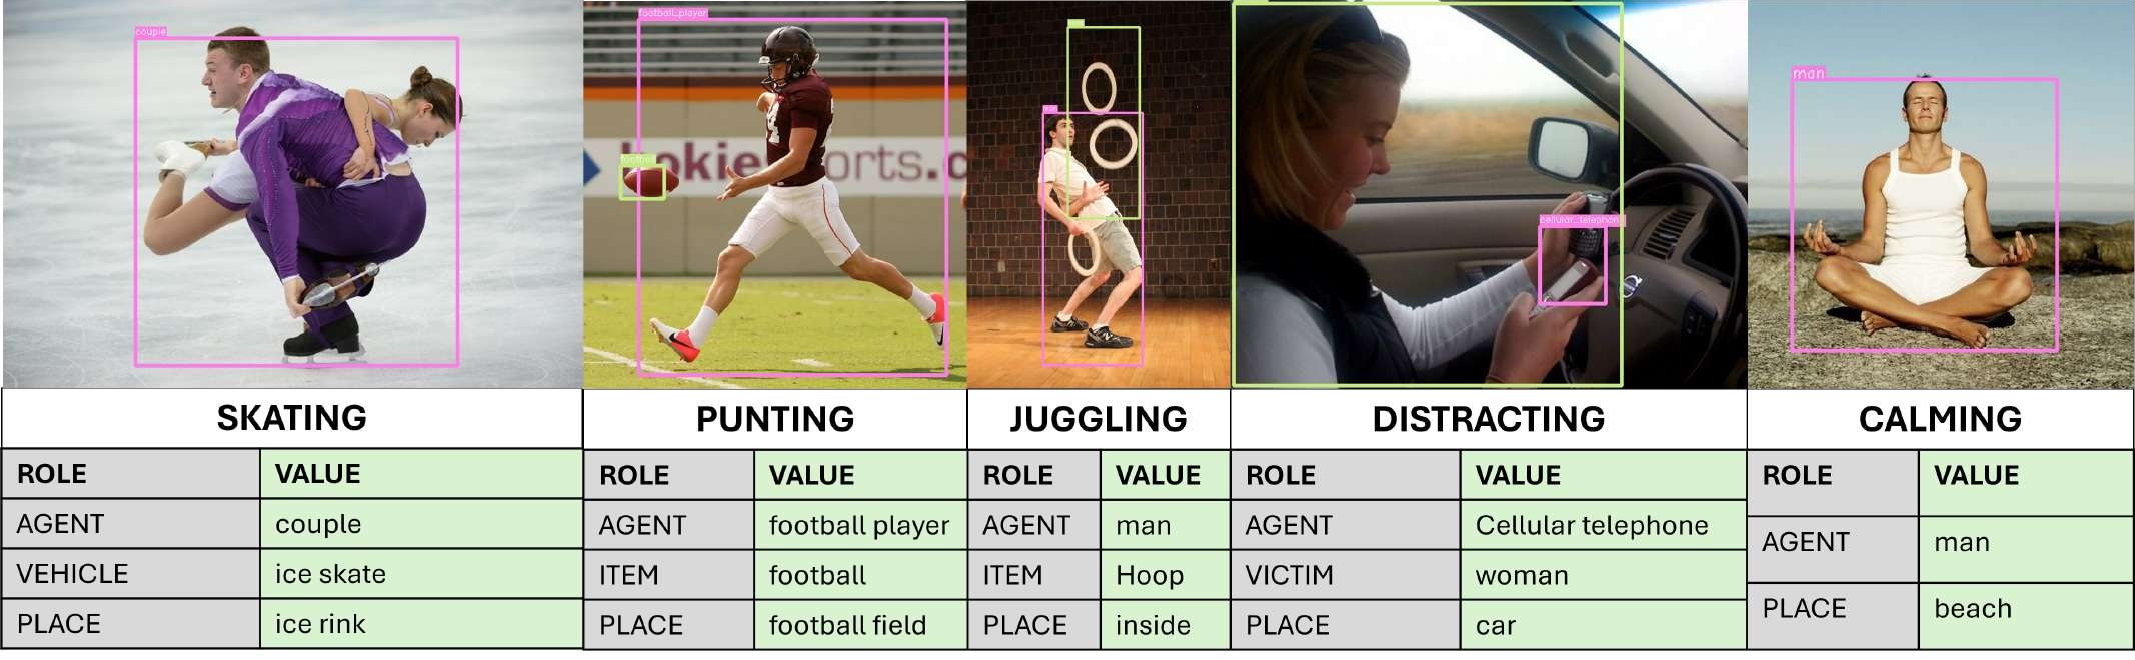
\includegraphics[width=0.99\textwidth]{figures/gsr_results.pdf}
    \caption{
    \textbf{Grounded Situation Recognition (GSR) qualitative results.} Results on the SWiG~\cite{pratt2020grounded} benchmark using our \attentionmethod method applied to CoFormer~\cite{cho2022collaborative}. The predicted main activity for image is indicated below it, while the corresponding predicted semantic roles (arguments) are displayed in the table, with nouns labeled according to their specific roles within the activity. Bounding boxes for the predicted AGENT are shown in \textcolor{VioletRed}{pink} and other predicted roles' boxes are shown in \textcolor{Green}{green}. As demonstrated, our method successfully predicts complex situations, including those involving non-human agents.
    }
    \label{fig:gsr_task_results} 
\end{figure*}
